\section{Modeling}
\label{sec:modeling}
In this part we present the framework and generative process of our model $\boldsymbol{CDOT}$ (Community Detection Model of Multi-interaction Over Time), which can observe the time information between users and communities.
\begin{figure*}[th]
	\centering
	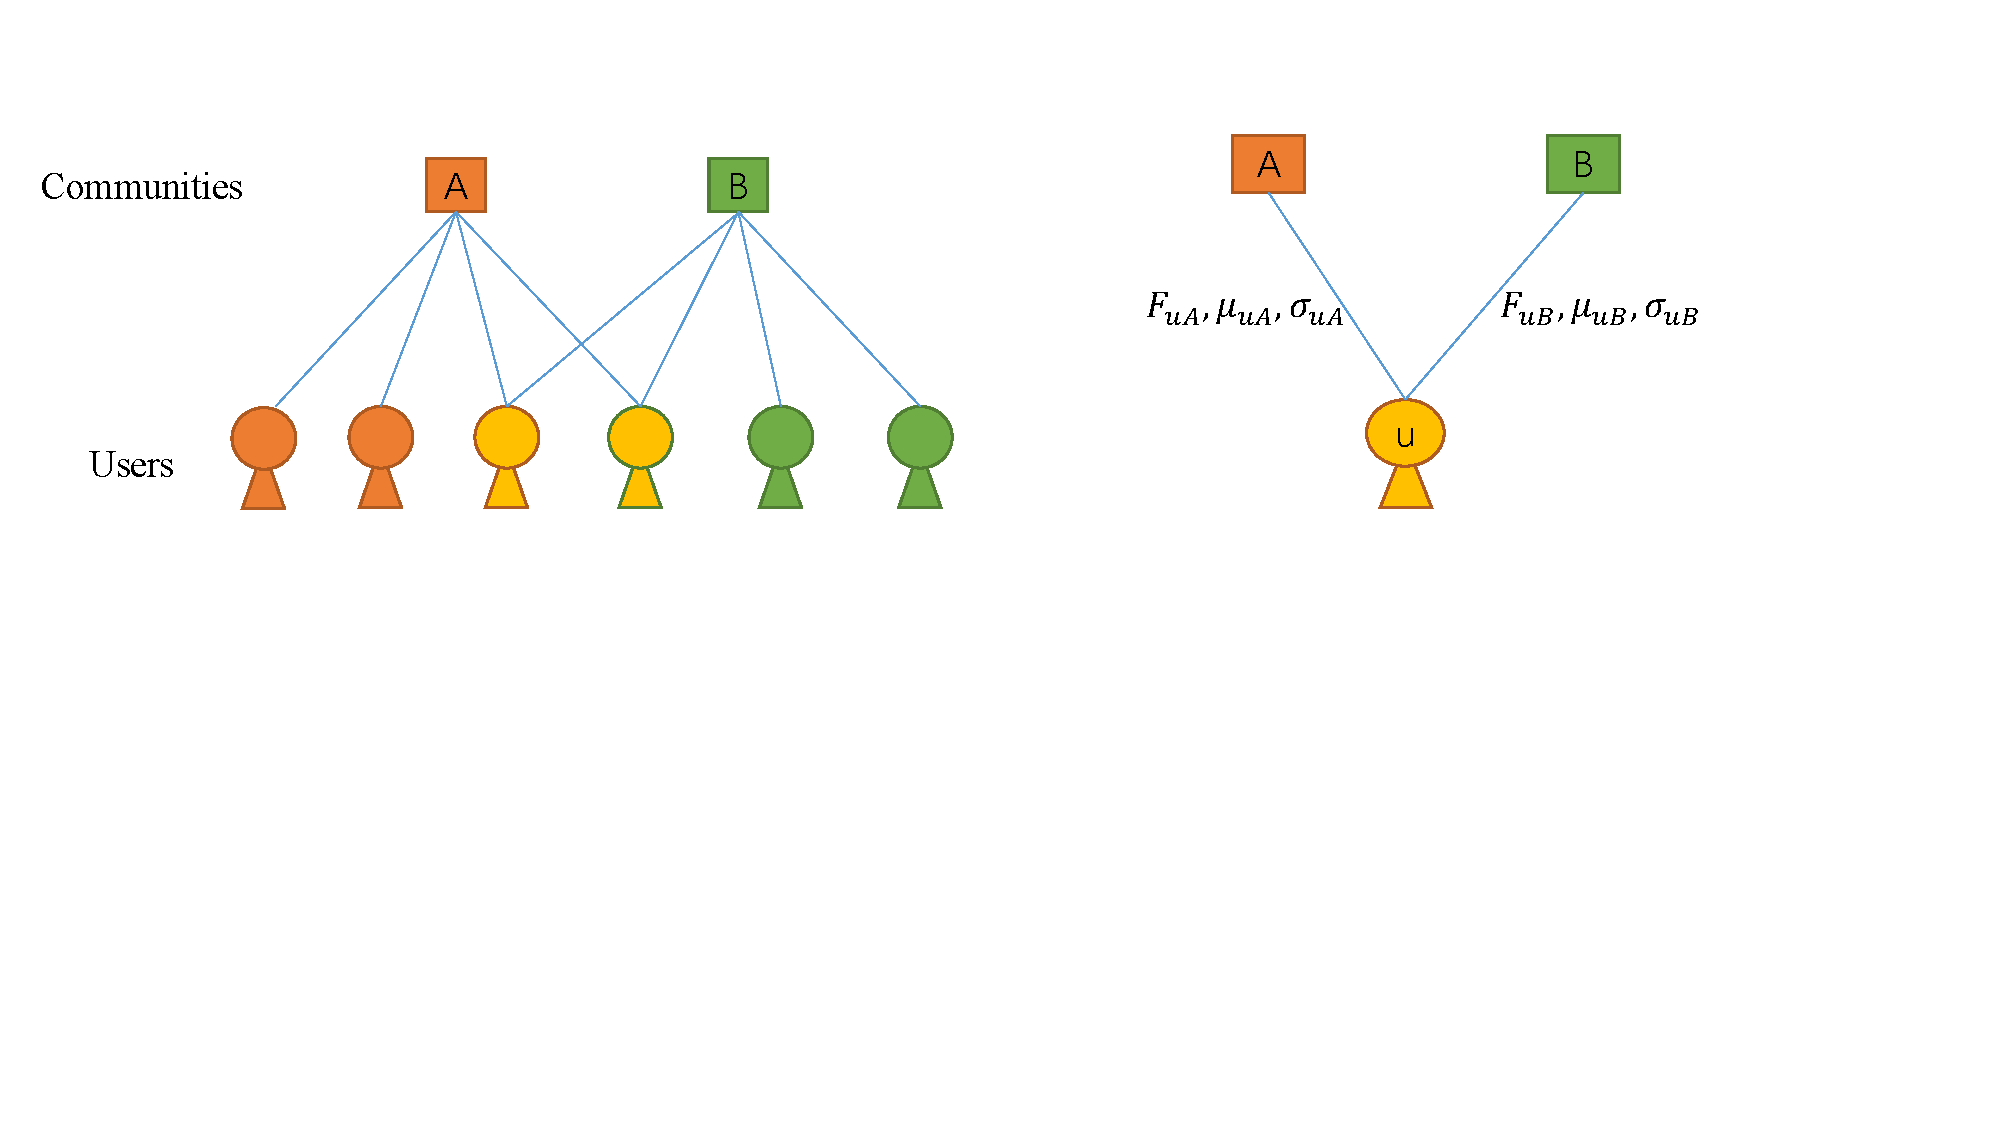
\epsfig{file=figures/model2.pdf, width=2\columnwidth}
	\caption{Bipartite affiliation graph. Each user will connect communities with a weight like $F_{uA}$ and a Guassian distribution with mean value $\mu_{uA}$ and variance $\sigma_{uA}$. }
	\label{fig:model2}
\end{figure*}
Fig. \ref{fig:model2} illustrates our model. Given a bipartite graph where the nodes at one side represent the nodes of the social network G, the nodes on the other side represent communities C, and the edge has three parameters, $F, \mu, \sigma$, the weight of the affiliation, mean value and variance of Guassian time distribution respectively.

\subsection{Model Description}
\label{subsec:formulation}





CDOT is based on the idea that communities arise due to shared group affiliation, and views the whole network as a result generated by a variant of the community-affiliation graph model. Same as the origin one, CDOT models the community affiliation strength between each pair of node u and community c with a nonnegative parameter $F_{uc}$($F_{uc}=0$ means node u is definitely not affiliated to community c.) 
However, CDOT also aim to detect $P_{uc}(t)$ which is a Guassian distribution between node u and community c over time t, so we consider that $F_{uc} P_{uc}$ is the community affiliation strength between node u and community c at time t.

We consider the input interaction network as a graph G(V,E) where V is a set of U users and E is a set of edges associated with two time stamps $t_1$ and $t_2$.

A directed edge $(u,t_1,v,t_2)$ means the interaction between user u and v and $t_1$ belongs to u and $t_2$ belongs to v, and there may be multiple edges between a pair of nodes, which means there are several interactions between them. Take dblp as an example, if one person u publish a paper at time $t_1$ and the person v cites it at time $t_2$, then they will have one edge between them.

To generate a link $(u(t_1), v(t_2))$ with probability $p(u,t_1,v,t_2)$, we define that:
\begin{equation}
\small
\begin{aligned}
p(u,v,t_1,t_2) =& 1-\exp(-\sum_{c=0}^{K}F_{uc}P_{uc}(t_1)F_{vc}P_{vc}(t_2))\\
P_{uc}(t_1) =& \frac{1}{\sqrt{2\pi}\sigma_{uc}}\exp(-\frac{(t_1-\mu_{uc})^2}{2\sigma_{uc}^{2}})\\
H=&\sum_{c=0}^{K}F_{uc}P_{uc}(t_1)F_{vc}P_{vc}(t_2)
\end{aligned}
\end{equation}
The process in Eq.1 suggests the possibility of node u in the time $t_1$ connects node v in the time $t_2$ within each community. There will be three parameter between node u and community c: $F_{uc}, \mu_{uc}, \sigma_{uc}$, where $F_{uc}$ denotes the total strength between them, $\mu_{uc}$ and $ \sigma_{uc} $ are the mean and variance value of Gaussian distribution, where $\mu_{uc}$ denotes the  maximum likelihood time of node u in the community c, and $\sigma_{uc}$ evaluate if the person is ``temporal'' to the community or ``stable'', which means that if $\sigma_{uc} \le \delta$ ($\delta $ is the threshold of temporal and stable), he is ``temporal'', belongs to the community at a special short period of time  near $\mu_{uc}$. If $\sigma_{uc} \textgreater \delta$, he is ``stable'', belongs to the community over a  long time.

$\delta$\textbf{-Threshold.} As shown in Fig. \ref{fig:model}. In the above we have defined a threshold of $\sigma$ determining if one node belongs to a community ``temporal'' or ``stable'', we find that if the $\sigma_{uc}$ satisfy the function that $P_{uc}(\mu_{uc})/P_{uc}(|\mu_{uc}-5|)> 0.5 $ it is ``temporal'', otherwise ``stable''.

\subsection{Community Detection Over Time}
\label{subsec:detection}
\begin{figure}[th]
	\centering
	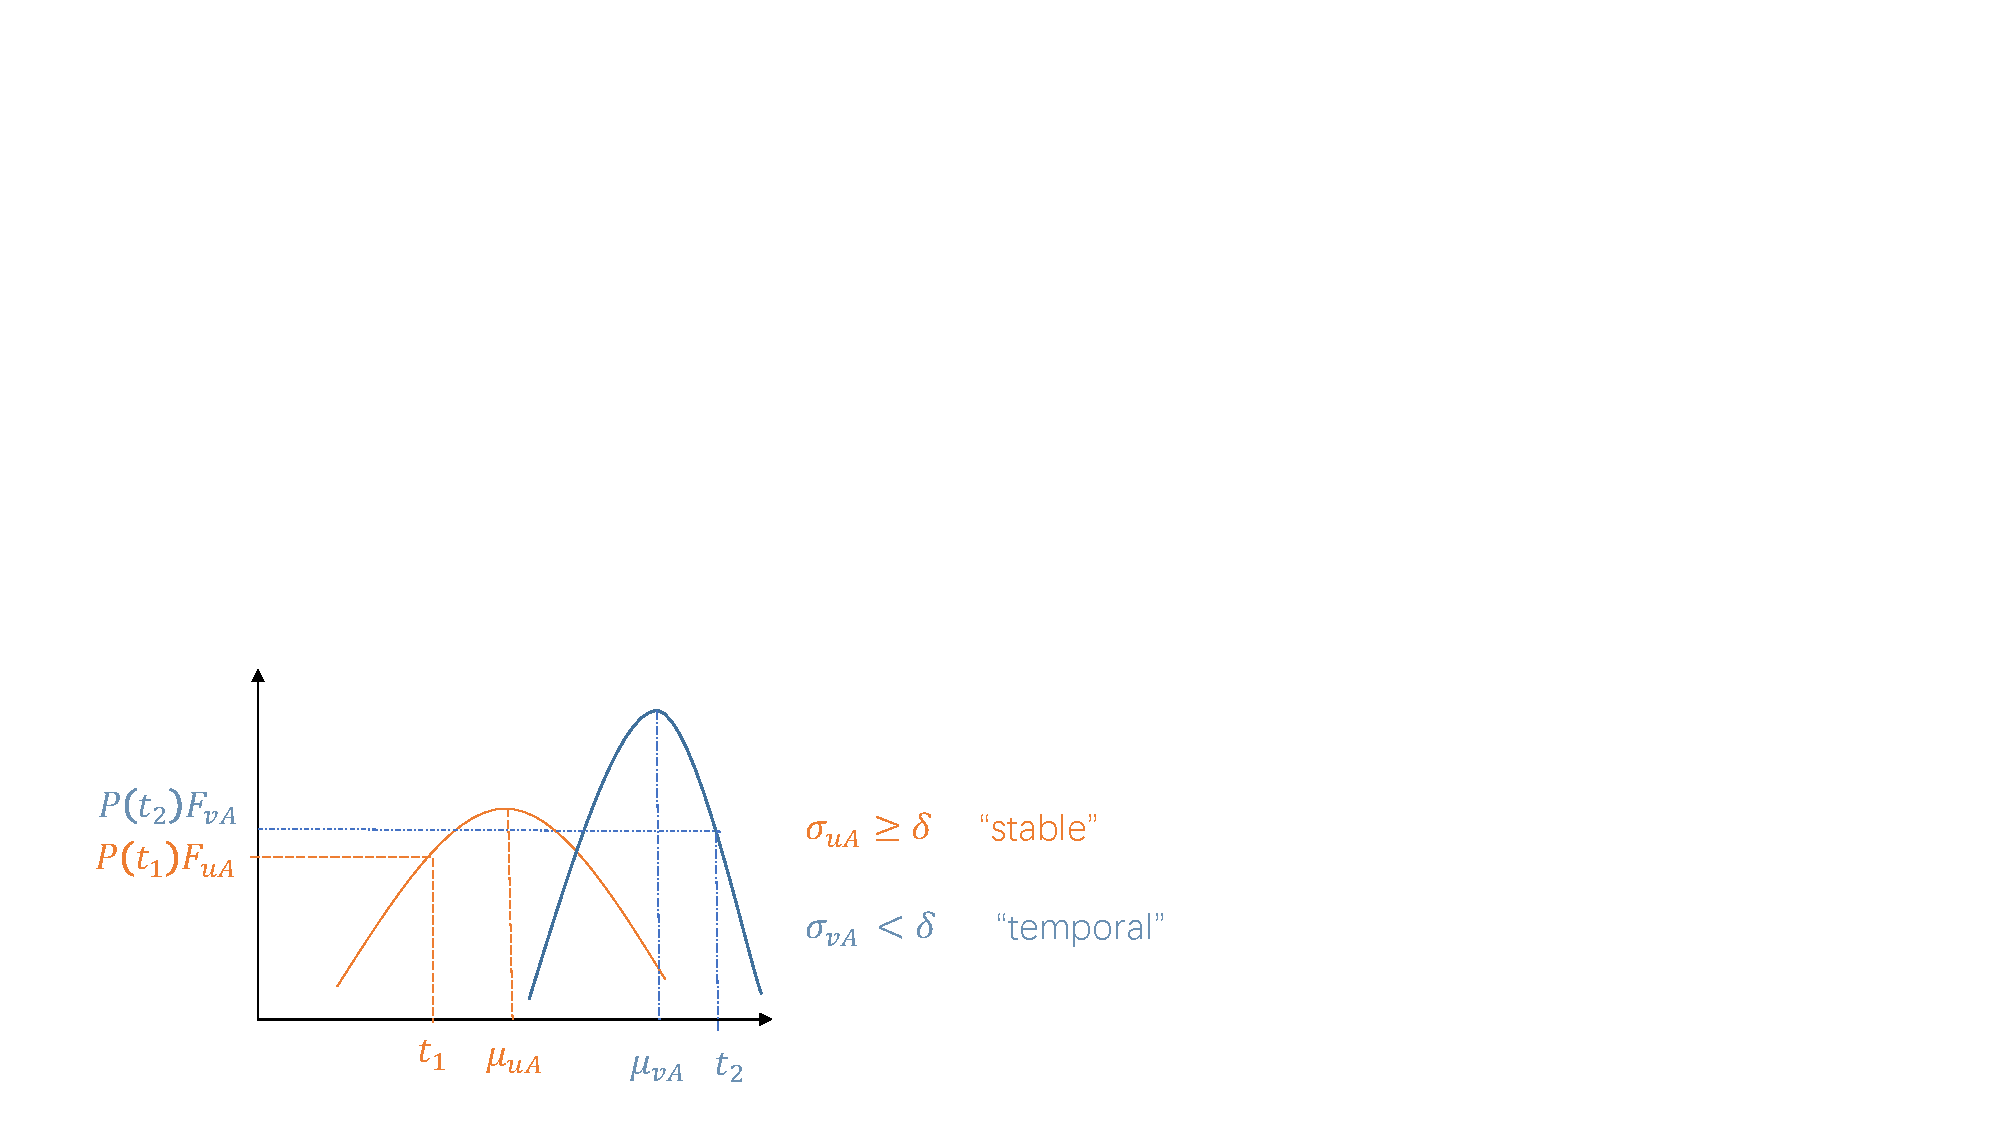
\epsfig{file=figures/model.pdf, width=\columnwidth}
	\caption{$\sigma_{uA} \ge \delta$: the node $u$ is ``stable'' to community $A$. $\sigma_{vA} \textless \delta$: the node $v$ is ``temporal'' to community $A$.}
	\label{fig:model}
\end{figure}
Now we have defined the CDOT model, we explain how to detect network communities using the model.  Given the interaction network G(V,E), we aim to detect K communities by fitting the CDOT to the underlying network G by maximizing the log likelihood $l(F,\mu,\sigma) =\log P(G|F,\mu,\sigma)$:
\begin{equation}
\small
\begin{aligned}
&\hat{F},\hat{\mu},\hat{\sigma} = \underset{F\ge 0,  \sigma\textgreater 0}{\arg\max}  l(F,\mu,\sigma)\\
\end{aligned}
\end{equation}
where 
\begin{equation}
\scriptsize
\begin{aligned}
l(F,\mu,\sigma) = \sum_{(u,v,t_1,t_2)\in E} log(1-\exp{(-H)})-\sum_{(u,v,t_1,t_2)\not\in E}H
\end{aligned}
\end{equation}
where H is defined in E.q(1)
As a matter of fact, we will notice that the second term here is infinity on number, because the time t is a continuous parameter, and the time $t_1, t_2$ is infinity. We decide to using sampling method to deal with this problem, sample some negative edges to be the second term. The detail of implementing will be explained in the next section.
